\chapter{USB}
V tejto kapitole si rozšírime znalosti fungovania USB, ktoré sme získali v sekcii~\ref{uvod:sec:zakl_pojmy}. Najprv si vysvetlíme ako prebieha komunikácia medzi USB zariadením a hostom, následne sa pozrieme na konfiguráciu USB zariadenia po pripojení na zbernicu, prejdeme si niektoré základné USB descriptory a ako posledné si ešte vysvetlíme základnú stavbu USB na Windowse.

\section{Komunikácia}
Detailný popis komunikácie a presunu dát po zbernici je opísaný v USB 2.0 špecifikácii v kapitole 5~\cite{usb_chap5}. My sa momentálne zameriame len na určité časti, ktoré sú potrebné pre našu prácu. Každé USB zariadenie v sebe obsahuje tzv. \textit{endpointy}~\cite{usb_chap5_endpoint} -- môžeme to považovať za akúsi koncovku komunikácie medzi hostom a zariadením. Koncepčne sa jedná o schopnosť zariadenia v sebe uchovať dáta (memory buffer). Ako už vieme z kapitoly~\ref{uvod:sec:zakl_pojmy}, komunikáciu riadi USB host, a tá prebieha práve pomocou týchto endpointov -- v prípade ak chce host poslať určité dáta zariadeniu, zapíše ich do jeho konkrétneho endpointu. V prípade ak chce zariadenie poslať určité dáta hostovi, zapíše si ich do daného endpointu, odkiaľ ich host potom prečíta.

\subsection*{Endpoint}
\label{kap02:sec:endpoint}
USB zariadenie typicky pozostáva z niekoľkých na sebe nezávislých endpointov. Každý endpoint je potom jednoznačne určený:
\begin{enumerate}
\item Adresou USB zariadenia -- tá je pridelená USB zariadeniu pri jeho konfigurácii v momente pripojenia na zbernicu.
\item Číslom endpointu -- unikátne číslo, ktoré určuje výrobca zariadenia.
\item Smerom prenosu dát -- host $\longrightarrow$ device alebo device $\longrightarrow$ host.
\end{enumerate}

Do momentu pokiaľ neprebehne konfigurácia USB zariadenia a jeho endpointov, sú endpointy s adresou inou ako 0 v neurčitom stave a nemusia byť pre hosta dostupné. Endpoint s adresou 0, inak nazývaný aj ako \uv{default endpoint} alebo \uv{Endpoint0}, slúži na nakonfiguranie daného USB zariadenia. Výrobca zariadenia je povinný poskytnúť aspoň 1 Endpoint0 pre každý smer pohybu dát, prípadne 1 Endpoint0 s možnosťou prenosu oboma smermi. Funkcie (USB zariadenia) môžu obsahovať aj ďalšie endpointy s adresou inou ako 0. Tieto endpointy slúžia na prenos dát špecifických pre dané zariadenie (napríklad na posielane inputu myši). Rôzne endpointy môžeme zlučovať do určitých množín podľa ich funkcionality. Takúto množinu endpointov potom nazývame \textit{interface}. Niektoré USB zariadenia potom môžu pozostávať z viacerých interfacov, ktoré budú reprezentovať rozličné USB triedy.

\subsection*{Pipe}
USB pipe~\cite{usb_chap5_pipe} je termín označujúci spojenie medzi konkrétnym endpointom USB zariadenia a Host Controllerom (interface medzi hostom a zbernicou). Reprezentuje schopnosť prenášať dáta medzi hostom a endpointom pomocou memory bufferu. Pipe ktorá pozostáva z dvoch Endpoint0 sa nazýva \uv{Default Control Pipe} a je prístupná v momente pripojenia zariadenia na zbernicu a slúži na konfiguráciu daného zariadenia (po konfigurácii môže mať aj iné využitie, ktoré špecifikuje samotný výrobca). Ostatné pipy s ďalšími endpointami (za predpokladu, že existujú) sú vytvorené až po konfigurácii zariadenia. 



\section{Konfigurácia}
Konfigurácia USB zariadenia je detailne opísaná v USB 2.0 špecifikácii~\cite{usb_chap9_conf}. Predtým ako začneme využívať funkcionalitu pripojeného USB zariadenia, je USB host zodpovedný za jeho nakonfigurovanie. Počas konfigurácie posiela USB host zariadeniu tzv. \uv{Device Requesty}, na ktoré dané zariadenie odpovedá cez Default Control Pipe. Tieto requesty sú špecifikované v \textit{Setup Pakete} -- štruktúra veľká 8 bytov so štandardným formátom definovaným v USB špecifikácii 2.0~\cite{usb_chap9_setup_pak}. Existuje niekoľko základných requestov~\cite{usb_chap9_device_req}, na ktoré musí každe USB zariadenie vedieť reagovať. Patria medzi ne napríklad:
\begin{itemize}
\item Get Descriptor -- vypýta si od zariadenia konkrétny descriptor, ktorý mu zariadenie pošle ako odpoveď na tento request (za predpokaldu, že daný descriptor existuje)
\item Set Configuration -- nastaví konkrétnu konfiguráciu zariadeniu
\end{itemize}

Bežný postup konfigurácie je, že si USB host vypýta rôzne descriptory od zariadenia, ktoré určujú jeho schopnosti (napr. \textit{Configuration Descriptor}, \textit{Interface Descriptor}, \textit{Endpoint Desriptor}) a potom pomocou requestu Set Configuration nastaví požadovanú konfiguráciu (a ak je to nutné, zvolí rôzne dodatočné nastavenie interfacov).



\section{USB Descriptory}
Teraz si prejdeme niekoľko základných USB descriptorov a ich jednotlivé položky, pretože ich význam budeme potrebovať neskôr v tejto práci. 


\subsection*{Configuration Descriptor}
Configuration Descriptor~\cite{usb_chap9_conf_desc} opisuje informácie o konkrétnej konfigurácii USB zariadenia. Obsahuje položku \textit{bConfigurationValue} -- číslo reprezentujúce konkrétnu konfiguráciu, ktorú USB host použije ako parameter v \texttt{SetConfiguration()} requeste v prípade, že chce nastaviť práve túto konfiguráciu. Každé zariadenie má aspoň jeden Configuration Descriptor. Každá konfigurácia obsahuje aspoň jeden interface a každý interface má nula alebo viac endpointov. V prípade, že si host vyžiada od zariadenia Configuration Descriptor, dostane spolu s ním aj všetky súvisiace Interface a Endpoint descriptory.


\subsection*{Interface Descriptor}
Interface Descriptor~\cite{usb_chap9_interf_desc} opisuje šepcifický interface konkrétnej konfigurácie USB zariadenia. Ak zariadenie podporuje viac ako jeden interface, tak všetky Interface Descriptory spolu s im odpovedajúcimi Endpoint Descriptormi sú vrátené ako odpoveď na \texttt{GetConfiguration()} request (k Interface Descriptoru nie je možný priamy prístup pomocou \texttt{GetDescriptor()} alebo \texttt{SetDescriptor()} requestom). Ak interface používa len Endpoint0, tak za Interface Descriptorom nenasleduje žiaden Endpoint Descriptor. Endpoint0 takisto nie je započítaný v položke Interface Descriptoru \textit{bNumEndpoints}, ktorá udáva počet endpointov konkrétneho interfacu.


\subsection*{Endpoint Descriptor}
Endpoint Descriptor~\cite{usb_chap9_end_desc} poskytuje hostovi informácie o konkrétnom endpointe. Tento descriptor obsahuje aj informácie na základe ktorých je host schopný určiť bandwidth konkrétneho endpointu -- množstvo dát prenesených za jednotku času (typicky bity za sekundu = b/s, alebo byty za sekundu = B/s). Takisto ako aj  pri Interface Descriptore, nie je možné k nemu priamo pristupovať pomocou \texttt{GetDescriptor()} alebo \texttt{SetDescriptor()} requestov, ale je súčasťou odpovede na \texttt{GetConfiguration()} request.

\section{Windows}
Keďže Windows je hlavná platforma na ktorú mierime s našou aplikáciou, priblížime si ako sú reprezentované jednotlivé USB zariadenia a priebeh komunikácie na danej zbernici.

Nasledujúca sekcia poskytuje zjednodušený popis a čerpá (pokiaľ nie je uvedené inak) z toho čo sa nachádza v Microsoft dokumentácii~\cite{usb_msdn_device_node_stack}.
Windows organizuje zariadenia pomocou stromovej štruktúry nazývanej \uv{Plug and Play device tree} alebo jednoducho len \uv{device tree}. Správca stromu sa nazýva \uv{PnP manager}~\cite{usb_msdn_pnp_manager}. Vrchol v tomto strome (tzv. \uv{device node}) reprezentuje USB zariadenie alebo nejakú jeho konkrétnu Funkciu. Koreň stromu obecne nazývame \uv{root device node} a typicky sa v diagramoch kreslí na spodku. Príklad takéhoto diagramu môžeme vidieť na obrázku~\ref{obr:kap2:device_tree} nižšie.

\begin{figure}[!htb]
	\centering
	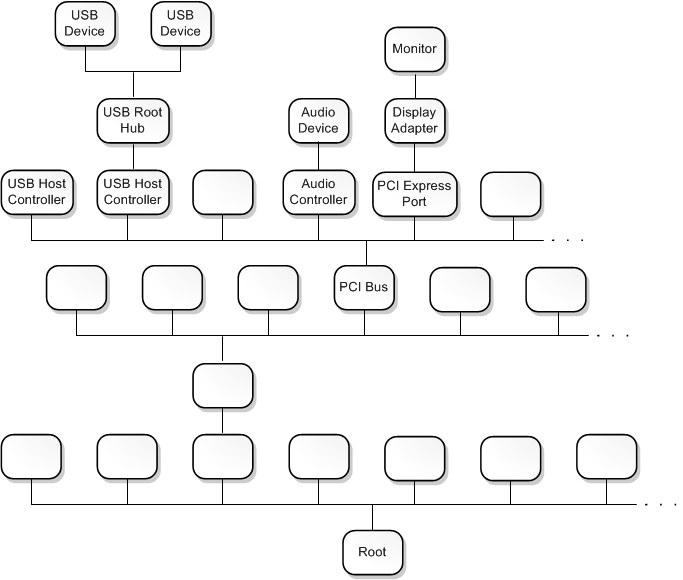
\includegraphics[width=10cm]{img/kap02_device_tree}
	\caption{Ukážka device tree. Obrázok prevzatý z Microsoft dokumentácie~\cite{usb_msdn_device_node_stack}}
	\label{obr:kap2:device_tree}
\end{figure}

Niektoré vrcholy môžu reprezentovať zbernice samotné, pričom synovia daného vrcholu zase reprezentujú zariadenia pripojené na túto zbernicu.

Windows má definovanú \texttt{DEVICE\_OBJECT} štruktúru~\cite{usb_msdn_device_object} reprezentujúcu \textit{device object} -- logické, virtuálne alebo fyzické zariadenie, ktoré využíva driver na spracovávanie I/O (input/output) requestov. Každý device node obsahuje usporiadaný list takýchto device objectov.  Usporiadaný list device objectov spolu s ich asociovanými drivermi nazývame \textit{device stack} (môžeme si to predstaviť ako stack dvojíc \textit{device object}$\leftrightarrow$driver). Tento stack má podľa konvencie vrch aj spodok -- prvé zariadenie ktoré bolo vytvorené na stacku sa nachádza na spodku a posledné vytvorené je naopak na vrchu. Ukážeme si to na konkrétnom príklade, kde na nasledujúcom obrázku~\ref{obr:kap2:device_node_diagram} môžeme vidieť device node s názvom \uv{Proseware Gizmo}, ktorého device stack obsahuje 3 položky: Vrchný device object má asociovaný \uv{AfterThought.sys} driver, stredný device object je spojený s driverom \uv{Proseware.sys} a posledný má zase \uv{Pci.sys} driver. Device stack \uv{PCI Bus} device nodu obsahuje len 2 položky: device node s \uv{Pci.sys} driverom a device node s \uv{Acpi.sys} driverom.

\begin{figure}[!htb]
	\centering
	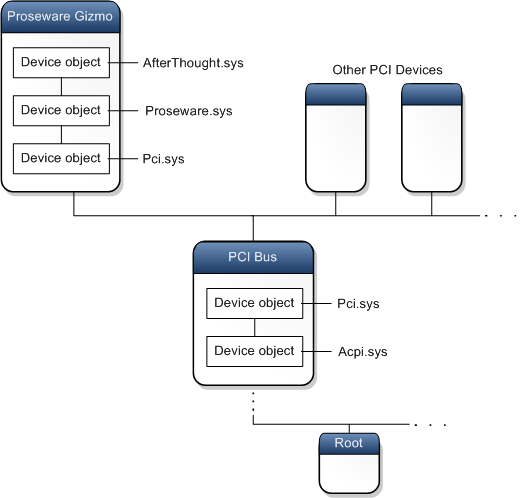
\includegraphics[width=10cm]{img/kap02_device_node_diagram}
	\caption{Ukážka konkrétnych device nodov. Obrázok prevzatý z Microsoft dokumentácie~\cite{usb_msdn_device_node_stack}}
	\label{obr:kap2:device_node_diagram}
\end{figure}

Konštrukcia tohto stacku je nasledovná:
\begin{itemize}
\item PnP manager poverí driver každej zbernice (v našom konkrétnom príklade z obrázku~\ref{obr:kap2:device_node_diagram} by to bol Pci.sys driver) aby sčítala všetky zariadenia, ktoré sú na ňu pripojené.
\item Ako odpoveď na túto požiadavku vytvorí driver danej zbernice device object pre každé pripojené zariadenie, ktorý nazývame \uv{physical device object (PDO)}. V príklade s Pci.sys driverom by to vyzeralo nasledovne:

\begin{figure}[!htb]
	\centering
	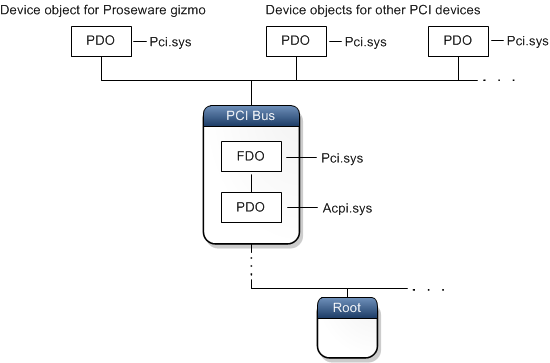
\includegraphics[width=10cm]{img/kap02_PDO}
	\caption{Ukážka vytvorenia konkrétnych PDO Pci.sys driverom. Obrázok prevzatý z Microsoft dokumentácie~\cite{usb_msdn_device_node_stack}}
	\label{obr:kap2:pdo}
\end{figure}

\item PnP manager pripradí device node každému novo vytvorenému PDO a pozrie sa do registru, aby zistil aké drivery majú byť súčasťou device stacku daného nodu. Každý device stack musí obsahovať práve jeden \textit{function driver} (hlavný driver device stacku, je zodpovedný za riadenie read, write a control requestov) a nula alebo viac \textit{filter driverov} (Ponúkajú prídavné možnosti v spracovávaní read, write a control requestov. Napríklad môžu meniť dáta, ktoré sú posielané daným requestom).
\item Akonáhle sú všetky drivery načítané, každý z nich vytvorí odpovedajúci device object a pripojí ho na daný device stack. Device object vytvorený function driverom nazývame \uv{functional device object (FDO)} a device objet vytvorený filter driverom zase \uv{filter device object (Filter DO)}. Náš konkrétny device tree vyobrazený na obrázku~\ref{obr:kap2:concrete_dev_tree} by teda vyzeral ako na obrázku~\ref{obr:kap2:concrete_dev_tree}.

\begin{figure}[!htb]
	\centering
	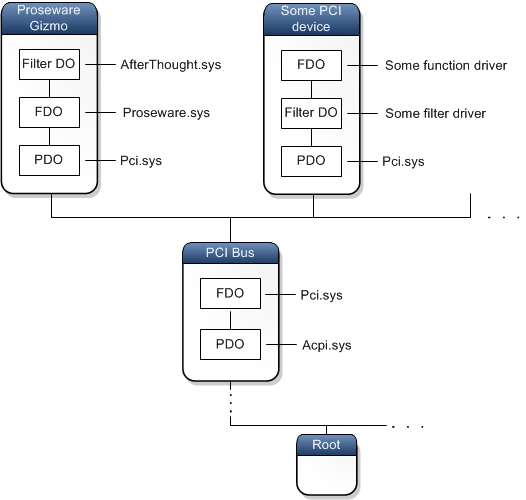
\includegraphics[width=10cm]{img/kap02_concrete_dev_tree}
	\caption{Ukážka konkrétneho device tree pre PCI zbernicu. Obrázok prevzatý z Microsoft dokumentácie~\cite{usb_msdn_device_node_stack}}
	\label{obr:kap2:concrete_dev_tree}
\end{figure}

\end{itemize}


Ako is ešte môžeme všimnúť na obrázku~\ref{obr:kap2:concrete_dev_tree}, v device node Proseware Gizmo je fitler driver (AfterThought.sys) nad function driverom (Proseware.sys). V takomto prípade je daný filter driver nazývaný \uv{upper filter driver}. Naopak v druhom device node (Some PCI device) je filter driver pod function driverom -- takýto filter driver nazývame \uv{lower filter driver}.

Keďže sú pre našu aplikáciu dôležité hlavne HID zariadenia, pozrieme sa teraz na to ako vyzerá driver stack a celková architektúra pre túto triedu zariadení~\label{kap02:sec:hid_arch}. Základom každého device stacku HID zariadenia je class driver \textit{hidclass.sys}, za ktorým nasledujú už konkrétne function/filter drivery. Príklad device stacku myši a klávesnice, tak ako aj HID triedy môžeme vidieť na nasledujúcom obrázku~\ref{obr:kap2:concrete_dev_stack}:

\begin{figure}[!htb]
	\centering
	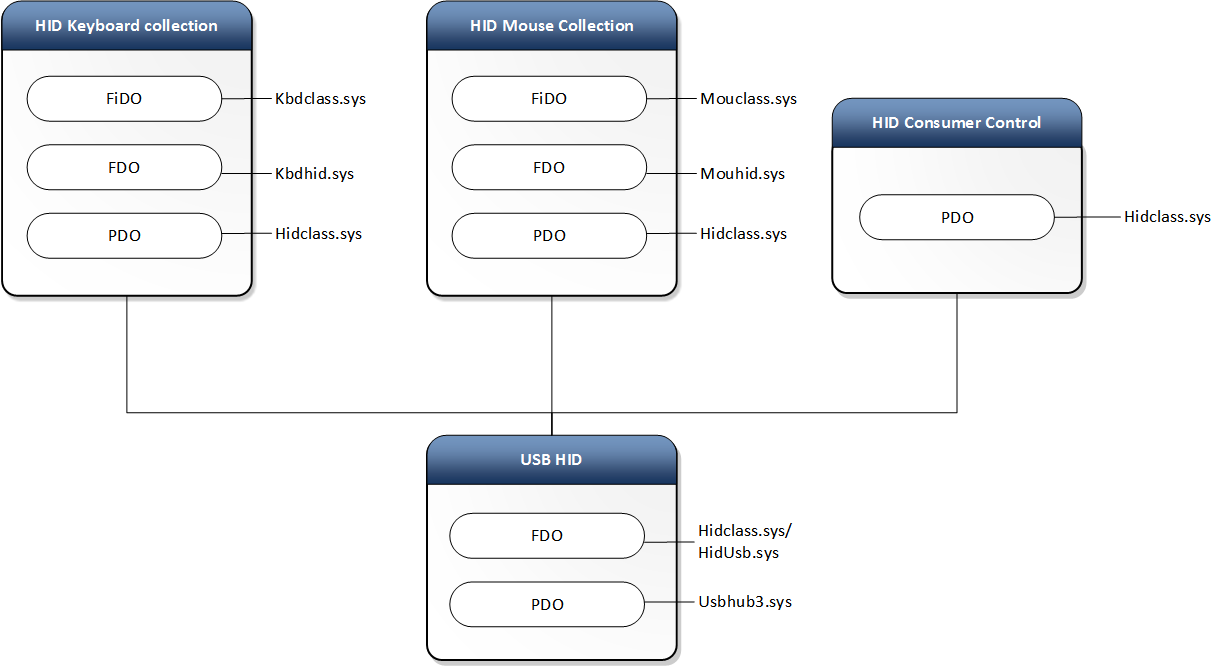
\includegraphics[width=\textwidth]{img/kap02_concrete_device_stack}
	\caption{Ukážka konkrétneho device stacku myši a klávesnice. Obrázok prevzatý z Microsoft dokumentácie~\cite{usb_msdn_hid_architecture}}
	\label{obr:kap2:concrete_dev_stack}
\end{figure}

Momentálne si vysvetlíme ešte zopár pojmov, ktoré sa nám budú hodiť neskôr v texte. \uv{HID Client}~\cite{usb_msdn_hid_client} je termín ktorým označujeme driver, service~\cite{usb_msdn_service} alebo aplikáciu, ktorá komunikuje s \textit{hidclass.sys} a často reprezentuje konkrétne zariadenie (napríklad myš alebo klávesnicu). \uv{Preparsed Data}~\cite{usb_msdn_preparsed_data} reprezentujú dáta Report Descriptoru asociované s konkrétnym zariadením. Aplikácie ich využívajú aby z nich vytiahli informácie o danom zariadení bez nutnosti parsovania Report Descriptoru.